\chapter{Solution Design}
\label{chp:solution-design}
The proposed solution builds on some of the advancements in the field of self-sovereign digital identity as shown in Section \ref{sec:blockchain-identity}. It focuses on a decentralised model of data storage and communication, with privacy-preserving features and identity recovery.

\section{System Overview}

The system is comprised of three primary parts:
\begin{enumerate}
	\item \textbf{Smart Contracts}: These are immutable programs stored on the Ethereum blockchain. Their function is to store the unique user identifier, a pointer to the user's data and the logic for modifying this data.
    \item \textbf{Data Storage}: The user data is stored in \ac{JSON} format on the decentralised storage platform \ac{IPFS}, with a reference to this data given to the smart contract.
	\item \textbf{Device Key Pair}: This is a public and private key pair stored on the end user's device, used for authenticating the user and allowing them to access and update their identity.
\end{enumerate}

\subsection{Smart Contracts}
The smart contracts are the core of the user's identity. There are two smart contracts that the user deploys onto the blockchain, that represent their identity.

The source code for these contracts is necessarily simple, to facilitate robust code execution and transparent auditing. This can be viewed in detail in Appendices \ref{apd:identity-contract} and \ref{apd:recovery-contract}.

\subsubsection{Identity Contract}
This contract contains the authoritative version of the user's identity, as well as the access control logic for attribute modification. Once this contract is deployed to the blockchain, the reference address that is returned is the user's \ac{UUID}. This address never changes, and it ensures the user maintains a persistent identifier even if their personal access keys are recovered or updated.
The data stored in the contract is shown in Table \ref{tab:identity-contract} below.

\begin{table}[h]
	\centering
    \begin{tabular}{|p{3cm}|p{8cm}|}
        \hline \textbf{Contract Data} & \textbf{Purpose} \\
        \hline owner\_key & Public key of the identity owner \\
        \hline recovery\_contract & Address of the associated recovery contract \\
        \hline ipfs\_hash & Hash pointing to the user data in \ac{IPFS} \\
        \hline
    \end{tabular}
    \caption{Identity contract storage variables}
    \label{tab:identity-contract}   
\end{table}

The \textit{owner\_key} value represents the public part of the user's key pair stored on their device. The \textit{recovery\_contract} value is the address of the recovery contract described below. Requests to change user data are only accepted if they come from the listed public key or recovery contract.

\subsubsection{Recovery Contract}
This contract contains the logic to restore access to a user's identity. It stores a list of the user's friends that have been selected to facilitate recovery.

\begin{table}[h]
	\centering
    \begin{tabular}{|p{2.5cm}|p{9cm}|}
        \hline \textbf{Contract Data} & \textbf{Purpose} \\
     	\hline uuid & Address of the user's identity contract \\
     	\hline contacts\_list & List of recovery contact addresses \\
    	\hline recoveries & List of recovery requests submitted by contacts \\
     	\hline
    \end{tabular} \\
    \caption{Recovery contract storage variables}
    \label{tab:recovery-contract}   
\end{table}

The \textit{uuid} is a pointer to the user's identity contract. The \textit{contacts\_list} stores \acp{UUID} of accounts selected by the user. Requests to change the contacts list can only be done via the listed identity contract address. The \textit{recoveries} value contains pending recovery requests for the identity, and it is cleared when a pending recovery is approved by a majority of peers.


\subsection{Identity Creation}
\begin{figure}[ht]
\centering
     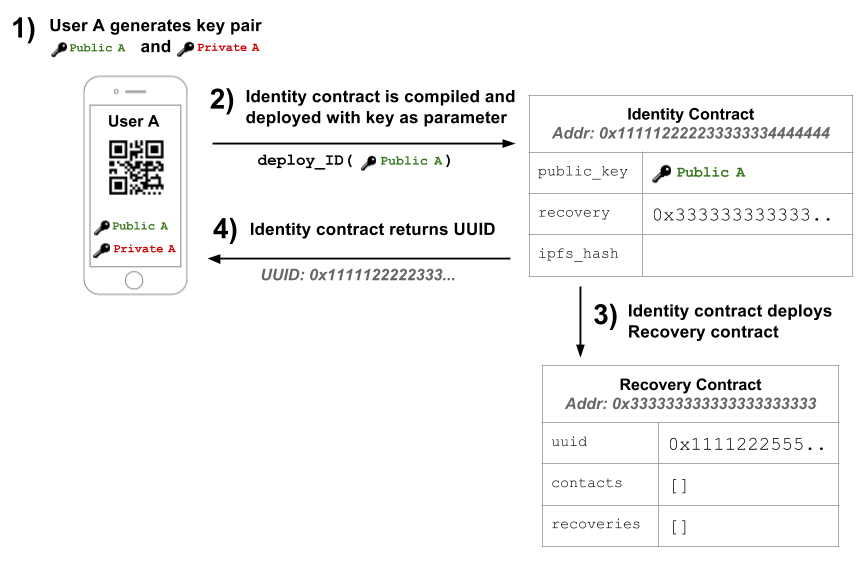
\includegraphics[width=1.0\textwidth]{./images/DiagramSignup.png}
      \caption{Identity Creation: Key generation and contract deploy steps.}
       \label{fig:diagram-signup}
\end{figure}

The steps for identity creation are shown in Figure \ref{fig:diagram-signup}. To create an identity on the platform, the user first generates a public and private key pair on their device. The public key acts as the local identifier for the user and is also an Ethereum address that can hold currency. The private key is used for signing transactions from this address, and to prove ownership of the public key.

The user then compiles a copy of the \textit{Identity Contract} source code and publishes it to the blockchain via their Ethereum address. This transaction returns the Ethereum address to which the contract was deployed, and is used as the unique identifier or \ac{UUID} for the user. 

This form of identifier is seen in the case of uPort in Section \ref{sec:uport}, and it is useful as it functions as both a unique address and a pointer to the contract data on the blockchain.

The identity contract itself also publishes a second contract, known as the \textit{Recovery contract}. This contains the storage and logic for identity recovery using a consensus of the user's selected friends.


\subsection{User Attributes}
These are descriptive attributes relating to the user, for example, their name, address or date of birth. These are stored as \ac{JSON} objects on the decentralised storage platform \ac{IPFS}. To store a user's attributes on their identity, they upload it to \ac{IPFS} and receive a resultant hash pointing to the content on the \ac{IPFS} network. The user can then send a signed transaction using their device public key to their identity contract which updates the \ac{IPFS} hash.

\subsection{Attribute Signing}
Information about a user is not useful unless it is verified by a trusted third party. A user can request that a third party signs their attributes, and can then save the resultant signature with the rest of their identity details. Signatures contain the requested attribute, the \ac{UUID} of the user, and a signature expiry time. 

Smart contracts currently cannot perform signing functions on arbitrary pieces of text, and therefore the signatures must be done using the private key on the third party's device. Signatures performed using device keys are accompanied by the associated contract address for subsequent verification.

There is, therefore, a link between the user's device keys and the \ac{UUID} value stored on the blockchain that must be consistently verified. All signed data must be checked against the blockchain to ensure that the public key used to sign is still matched with the correct identity.

\subsection{Attribute Disclosure}
\label{sec:attribute-disclosure}
\begin{figure}[ht]
\centering
     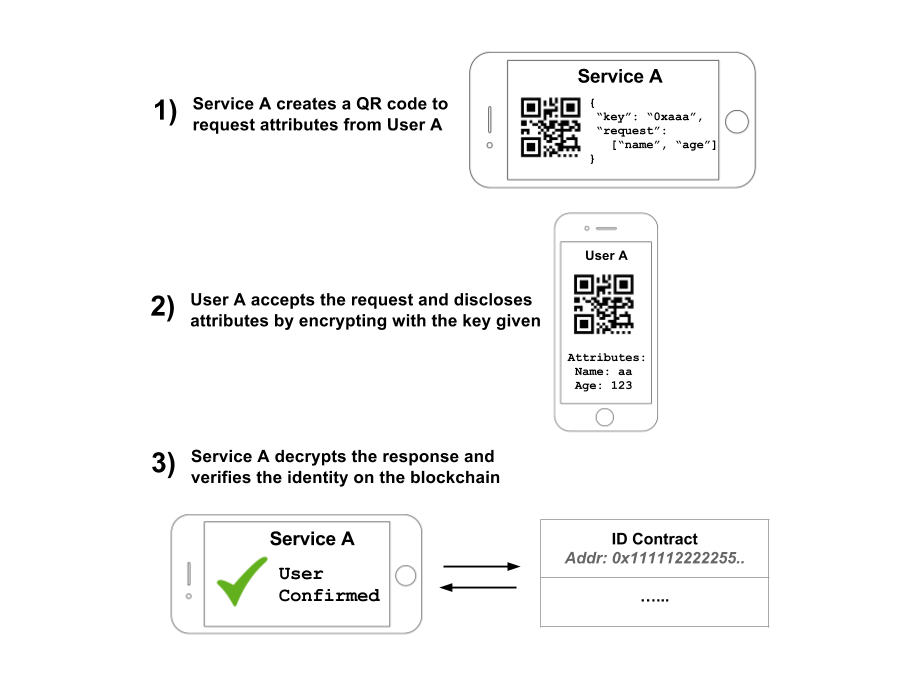
\includegraphics[width=1.0\textwidth]{./images/DiagramDisclosure.png}
      \caption{Attribute Disclosure: Steps to disclose user attributes to a third party.}
       \label{fig:diagram-disclosure}
\end{figure}
To disclose a user's attributes to another party, the third party service creates a disclosure request with the required attributes. This is shown in the first step of Figure \ref{fig:diagram-disclosure}. When the user receives this request on the device, they can confirm or deny the disclosure of the requested data.

The user then encrypts the attributes and any associated signatures with the third party's public key. The user also signs the request with the private key on their device and sends over the result.

The receiving party then decrypts this message and verifies that the public key used to create the signature is linked to the correct identity on the blockchain. The validity of any attribute signatures is also verified by querying the blockchain and checking that the signing parties are trusted.

Attributes of a user can only be considered valid if they are accompanied by attestations from third parties that are trusted by the receiver. An extension to this solution would allow a chain of trust to be created that links entities to trusted roots. Listing the public keys of trusted parties on an online service like the MIT PGP Public Key Server \cite{massachusetts_institute_of_technology_mit_nodate} could facilitate this approach.

\subsection{Identity Recovery}
\label{sec:identity-recovery}
\begin{figure}[ht]
\centering
     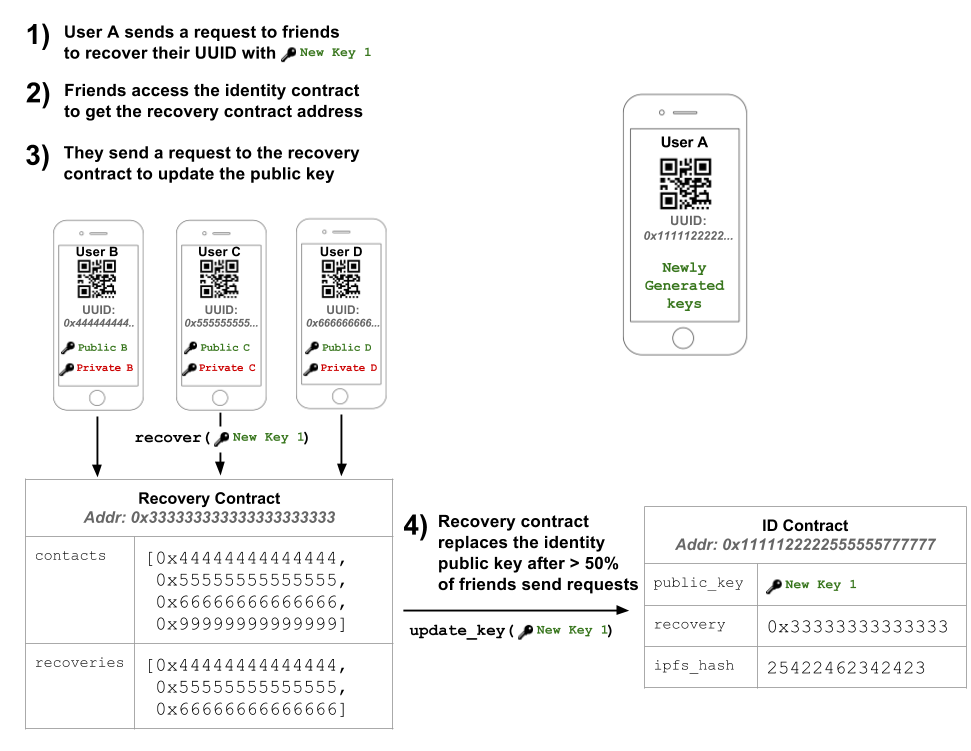
\includegraphics[width=1.0\textwidth]{./images/DiagramRecovery.png}
      \caption{Identity Recovery: Steps to recover an identity using a network of trusted peers.}
       \label{fig:diagram-recovery}
\end{figure}

Recovery is a vital part of enabling public key cryptography for general use \cite{microsoft_key_nodate}.
In this approach, users preselect a group of recovery contacts to facilitate reinstatement of the user's identity in the event of key loss or compromise. The list of contacts are stored in the recovery contract connected to the user's identity. 

If a user needs to recover their identity, they first generate a new set of public and private keys. This can be seen in Step 1 of Figure \ref{fig:diagram-recovery} above. The user then meets with their contacts and asks them to send recovery requests containing their new public key.

The contacts then access the user's associated identity contract to get the address of the recovery contact before sending the request. The recovery contract stores pending requests, and has the power to make the key change once a majority decision is reached.

\subsection{Key Revocation}
Key revocation is used to permanently retire signing and encryption keys from usage \cite{brooks_key_1995}. In the context of key loss or compromise, this is an essential function to prevent malicious actors from abusing the system.

As the user's identity contract and \ac{UUID} is inherently tied directly to their device public key, this is the only valid mapping between these two values. This mapping is verified upon each signature and disclosure request, so separate key revocation does not need to be built into the system.

Key rotation within a user's identity should be logged for archival purposes, so that expired signatures can be verified as being valid at some point in the past. This can be achieved with Ethereum Event Logs \cite{chow_technical_2016}, which act as a logging tool for smart contracts that is cheaper than internal storage. Parties can subscribe to the outputs of these events and be notified when they are announced.

The invalidation of old signatures when an identity has its keys rotated is necessary to maintain the integrity of the identity network. New valid signatures should be distributed to appropriate parties when a relevant key change occurs.